\subsection*{Partie I. Exemples. Une inégalité générale.}

Dans toute cette partie, on utilisera souvent le r\'{e}sultat suivant.

\begin{quote}
Si une fonction continue, d\'{e}finie dans $\R$ est monotone au
voisinage de $+\infty $ et de $-\infty $ alors elle major\'{e}e si et
seulement si elle ne diverge pas vers $+\infty $ ni en $-\infty $ ni en $+\infty $.
\end{quote}

Ce r\'{e}sultat est une cons\'{e}quence des d\'{e}finitions des limites et du fait qu'une fonction continue sur un segment est born\'{e}e$.$

\begin{enumerate}
\item Ici $X=\R$, $f(x)=Kx^{2}$, $h_m(x)=mx-Kx^2$.
\begin{itemize}
 \item Si $K<0$, $h_m$ n'est majorée pour aucune valeur de $m$.
 \item Si $K>0$, $h_m$ est majorée pour tous les $m$ réels. On obtient facilement la valeur minimale de la fonction du second degré. On en déduit :
\begin{displaymath}
 X^\circ =\R ;\; f^\circ (m)=\dfrac{m^2}{4K}
\end{displaymath}
On vérifie que $f=f^\circ$ si et seulement si $K=\frac{1}{2}$.
\end{itemize}

\item  Lorsque $f$ est une fonction continue sur un segment $X=\left[a,b\right] $, il en est de m\^{e}me des fonctions $h_{m}$ pour n'importe quelle valeur de $m$. Ces fonctions sont donc toujours born\'{e}es ce qui montre $X^\circ =\R$ \newline
Chaque fonction continue $h_{m}$ atteint ses bornes sur le segment $\left[ a,b\right] $. Il existe donc $x_{m}\in \left[a,b\right]$ tel que $f^{\circ }(m)=h_{m}(x_{m})$. Dans ce cas rien n'assure l'unicité de $x_m$.

\item  Ici $X=\R$ et $f(x)=\frac{1}{3}x^{3}$. Comme $h_{m}(x)=mx-\frac{1}{3}x^{3}$, elle est monotone au voisinage de $+\infty $ et de $-\infty $ avec
\[
h_{m}(x)\sim -\frac{1}{3}x^{3}
\]
Cette fonction diverge vers $+\infty $ en $-\infty $. Elle n'est pas born\'{e}e par cons\'{e}quent
\[
X^{\circ }=\emptyset
\]

\item  Ici $X=\R$ et 
\[f(x)=e^{x} , h_{m}(x)=mx-e^{x}\]
Examinons les limites 
\begin{eqnarray*}
\text{en }-\infty  &:&\quad h_{m}(x)\rightarrow \left\{
\begin{array}{ccc}
-\infty  & \text{si} & m>0 \\
0 & \text{si} & m=0 \\
+\infty  & \text{si} & m<0
\end{array}
\right.  \\
\text{en }+\infty  &:&\quad h_{m}(x)\rightarrow -\infty
\end{eqnarray*}
Le r\'{e}sultat pr\'{e}cis\'{e} au début permet de conclure que $X^{\circ }=\left[ 0,+\infty \right[ $.\newline
Si $m=0$, la fonction $h_{0}(x)=-e^{x}$ admet $0$ comme borne sup\'{e}rieure donc $f^{\circ }(0)=0$.\newline
Si $m>0$, formons le tableau de variations de $h_{m}(x)=mx-e^{x}$.\newline
On a $h_{m}^{\prime }(x)=m-e^{x}$ et
\[
\begin{array}{c|ccccc}
& 0 &  & \ln m &  & +\infty  \\
\hline
&  &  & m\ln m-m &  &  \\
h_{m} &  & \nearrow  &  & \searrow  &  \\
& -1 &  &  &  & -\infty
\end{array}
\]
On en d\'{e}duit (en notant \`{a} nouveau $x$ la variable)
\begin{eqnarray*}
X^{\circ } &=&\left[ 0,+\infty \right[  \\
f^{\circ }(x) &=&\left\{
\begin{array}{ccc}
0 & \text{si} & x=0 \\
x\ln x-x & \text{si} & x>0
\end{array}
\right.
\end{eqnarray*}
On forme alors $k_{u}(x)=ux-x\ln x + x$ pour $x>0$ dont on cherche le tableau de variations $k_{u}^{\prime }(x)=u-\ln x$ :
\[
\begin{array}{c|ccccc}
& 0 &  & e^{u} &  & +\infty  \\
\hline
&  &  & e^{u} &  &  \\
k_{u} &  & \nearrow  &  & \searrow  &  \\
& 0 &  &  &  & -\infty
\end{array}
\]
On en d\'{e}duit $X^{\circ \circ }=\R$ avec $f^{\circ \circ}(x)=e^{x}$.

\item  Ici $X=\R$ et $f(x)=\alpha x+\beta $, $h_{m}(x)=mx-\alpha x-\beta =(m-\alpha )x-\beta $. Si $m\neq \alpha ,$ une des limites en $\pm \infty $ est $+\infty $ et donc $h_{m}$ n'est pas major\'{e}e$.$ On en d\'{e}duit
\[
X^{\circ }=\left\{ \alpha \right\} ,\quad f^{\circ }(\alpha)=-\beta
\]
Alors $h_{u}$ est toujours born\'{e}e puisque son domaine de d\'{e}finition est r\'{e}duit au seul point $\alpha $ avec $h_{u}(\alpha )=u\alpha -(-\beta )$. Donc en revenant \`{a} la lettre $x$ pour d\'{e}signer la variable :
\[
X^{\circ \circ }=\R,\quad f^{\circ \circ }(x)=\alpha x+\beta
\]

\item  Ici $X$ ne contient que quatre points $X=\left\{ -1,0,1,2\right\}$ et
\[
h_{m}(x)=\left\{
\begin{array}{ccc}
-m-1 & \text{si} & x=-1 \\
0 & \text{si} & x=0 \\
m-2 & \text{si} & x=1 \\
2m-1 & \text{si} & x=2
\end{array}
\right.
\]
La question est alors de savoir, pour un nombre $m$ donn\'{e}, quel est le plus grand des quatre nombres
\begin{align*}
 -1-m & & 0 & & m-2 & & 2m-1
\end{align*}
Le plus commode est de faire une étude graphique en traçant les quatre droites 
\begin{align*}
 m\rightarrow -1-m & & m\rightarrow 0 & & m\rightarrow m-2 & & m\rightarrow 2m-1
\end{align*}
Une de ces droites est l'axe des $x$. On voit clairement sur le dessin le graphe de $f^\circ$ et on déduit facilement son expression (la démonstration ne mérite pas vraiment qu'on s'y attarde).
\begin{figure}
   \centering
   \input{Cdualsup_1.pdf_t}
   \caption{I.6. \'Etude graphique}
   \label{fig:Cdualsup_1}
\end{figure}
On en d\'{e}duit $X^{\circ }=\R$ et, en notant \`{a} nouveau $x$ la variable,
\[
f^{\circ }(x)=\left\{
\begin{array}{ccc}
-x-1 & \text{si} & x\leq -1 \\
0 & \text{si} & x\in \left[ -1,\frac{1}{2}\right]  \\
2x-1 & \text{si} & x\geq \frac{1}{2}
\end{array}
\right.
\]
Il est important de noter que la fonction $f^{\circ }$ est continue. Formons maintenant $k_{u}(x)$
\[
k_{u}(x)=\left\{
\begin{array}{ccc}
ux-(-x-1)=(u+1)x+1 & \text{si} & x\leq -1 \\
ux-0=ux & \text{si} & x\in \left[ -1,\frac{1}{2}\right]  \\
ux-(2x-1)=(u-2)x+1 & \text{si} & x\geq \frac{1}{2}
\end{array}
\right.
\]
\`A cause du r\'{e}sultat cit\'{e} dans le pr\'{e}ambule, la fonction $k_{u}$ est major\'{e}e si et seulement si $u+1\geq 0$ et $u-2\leq 0$. Par cons\'{e}quent $X^{\circ \circ }=\left[ -1,2\right] $.\newline
Sur $\left] -\infty ,-1\right] $ la fonction $k_{u}$ est croissante. Elle atteint sa borne sup\'{e}rieure en $-1$ en prenant la valeur $-u$.\newline
Sur $\left[ \frac{1}{2},+\infty \right[ $ la fonction $k_{u}$ est d\'{e}croissante. Elle atteint sa borne sup\'{e}rieure en $\frac{1}{2}$ en prenant la valeur $\frac{u}{2}$.\newline
Sur $\left[ -1,\frac{1}{2}\right] $ la fonction $k_{u}$ est affine et varie
entre les deux valeurs pr\'{e}cedentes. Sa borne sup\'{e}rieure est donc la plus grande des deux valeurs pr\'{e}c\'{e}dentes.On en d\'{e}duit 
\begin{displaymath}
 \forall u\in \left[ -1,2\right]  : f^{\circ \circ }(u)=\sup_{\R}k_{u}=\max (-u,\frac{u}{2})
\end{displaymath}
Soit, revenant \`{a} la lettre $x$ :
\[
f^{\circ \circ }(x)=\left\{
\begin{array}{ccc}
-x & \text{ si } & x\in \left[ -1,0\right]  \\
\frac{1}{2}x & \text{si} & x\in \left[ 0,2\right]
\end{array}
\right.
\]
\begin{figure}
   \centering
   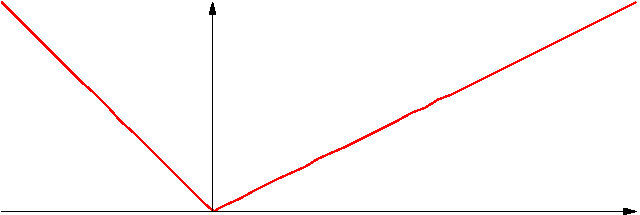
\includegraphics{Cdualsup_3.pdf}
   \caption{I.6. Graphe de $f^{\circ \circ}$}
   \label{fig:Cdualsup_3}
\end{figure}
On remarque que le domaine de d\'{e}finition est le plus petit intervalle contenant le domaine de d\'{e}finition de $f$.

\item  Pour $x\in X$ et $m\in X^{\circ }$, 
\begin{displaymath}
 mx-f(x)=h_{m}(x)\leq f^{\circ
}(m)=\sup_{X}h_{m}
\end{displaymath}
 d'o\`{u}
\[
mx\leq f(x)+f^{\circ }(m)
\]

\end{enumerate}

\subsection*{Partie II. Un autre exemple. Inégalité de Hölder.}
\begin{enumerate}
\item L'étude de la fonction $h_m$ conduit à $X^\circ=\R$ avec
\begin{displaymath}
 u_p^\circ(m)=0 \text{ pour } m\leq 0 \text{ et } u_p^\circ(m)=u_q(m) \text{ pour } m>0
\end{displaymath}
Au cours de cette étude on utilise en particulier la définition de $q$:
\begin{displaymath}
 1+\frac{1}{p-1}=\frac{p}{p-1}=\frac{1}{1-\frac{1}{p}}=q
\end{displaymath}

\item \begin{enumerate}
\item On exploite l'inégalité I.7. pour obtenir la première inégalité demandée puis on remplace $x$ par $\lambda x$ et $y$ par $\frac{1}{\lambda}y$ pour obtenir la seconde.
\item On ajoute les inégalités précédentes pour les couples $x_i$, $x_j$.
\end{enumerate}
\item
\begin{enumerate}
\item Calculons la dérivée de $v$:
\begin{displaymath}
 v'(x)=ax^{p-1}-bx^{-q-1}=ax^{-(1+q)}\left(x^{p+q}-\frac{b}{a} \right) 
\end{displaymath}
La fonction $v$ est donc décroissante puis croissante, elle atteint sa valeur minimale (notée $V$) en $(\frac{b}{a})^{\frac{1}{p+q}}$ avec 
\begin{displaymath}
 V = \frac{a}{p}(\frac{b}{a})^{\dfrac{p}{p+q}}+\frac{b}{q}(\frac{b}{a})^{-\dfrac{q}{p+q}}
\end{displaymath}
De plus,
\begin{displaymath}
\left. 
\begin{aligned}
 1-\frac{p}{p+q}=\frac{q}{p+q}=\frac{1}{p}\\
 1-\frac{q}{p+q}=\frac{p}{p+q}=\frac{1}{q}
\end{aligned}
\right\rbrace 
\Rightarrow
V=\frac{1}{p}a^{\frac{1}{p}}b^{\frac{1}{q}}+\frac{1}{q}a^{\frac{1}{p}}a^{\frac{1}{q}}
=a^{\frac{1}{p}}b^{\frac{1}{q}}
\end{displaymath}

\item L'inégalité du 2.b. est de la forme
\begin{displaymath}
 \forall \lambda>0, \sum_{i=1}^nx_iy_i\leq v(\lambda)\text{ avec }a=\sum_{i=1}^nx_i^p\text{ et }
b=\sum_{i=1}^ny_i^q
\end{displaymath}
On en déduit la meilleure inégalité possible $\sum_{i=1}^nx_iy_i\leq V$ où $V=a^{\frac{1}{p}}b^{\frac{1}{q}}$ est la valeur minimale de la fonction. On obtient ainsi l'inégalité de Hölder.
\end{enumerate}
 
\end{enumerate}
\subsection*{Partie III. Espaces $\mathcal{N}$ et $\mathcal{N}_0$ de fonctions convexes.}
Les conditions imposées aux fonctions de $\mathcal{N}$ et $\mathcal{N}_0$ entraînent clairement qu'elles sont convexes et croissantes.
\begin{enumerate}
\item Comme $f(0)=0$, on peut poser $\tau(x)=\frac{f(x)}{x}$ et interpréter $\tau$ comme le taux d'accroissement en 0 de la fonction $f$. D'après le théorème des accroissements finis, il existe $c_x \in ]0,x[$ tel que $\tau(x)=f'(c_x)$. Comme $\tau$ diverge vers $+\infty$, la fonction $f'$ n'est pas majorée, comme $f'$ est strictement croissante, elle diverge vers $+\infty$.
\item Appliquons le théorème des accroissements finis entre $x$ et $2x$.\newline
Il existe $c\in]x,2x[$ tel que
\[f(2x)-f(x)=xf'(c)\geq xf'(x)\]
car $f'$ est croissante. Comme de plus $f$ est aussi croissante avec $f(0)=0$, le nombre $f(x)$ est positif donc
\[xf'(x)\leq f(2x)\]
\item On suppose ici que $f'\rightarrow +\infty$ en $+\infty$. Comme
\[f'(x)\leq 2 \frac{f(2x)}{2x}\]
On en déduit $\frac{f(2x)}{2x}\rightarrow +\infty$. Comme d'autre part $\tau$ est croissante car $f$ est convexe, cela prouve que $\tau \rightarrow +\infty$
\end{enumerate}

\subsection*{Partie IV. Transformée de Legendre dans $\mathcal{N}_0$.}
\begin{enumerate}
\item Les propriétés des fonctions dans $\mathcal{N}_0$  en particulier $f'$ croissante, $f'\rightarrow +\infty$ en $+\infty$ et le calcul de $h'_m(x)=m-f'(x)$ conduisent au tableau suivant
\[
\begin{array}{c|ccccc}
& 0 &  & x_m &  & +\infty  \\
\hline
&  &  & f^{\circ}(m) &  &  \\
h_{m} &  & \nearrow  &  & \searrow  &  \\
& 0 &  &  &  & -\infty
\end{array}
\]
La fonction $h_m$ atteint son maximum en un unique point $x_m$ noté $\varphi(m)$.
\item \begin{enumerate}
\item Les conditions de $\mathcal{N}_0$ entraînent que $f'$ est strictement croissante de $\R_+$ dans $\R_+$. Elle est bijective car continue avec les \og bonnes limites\fg.
\item Comme $x_m$ annule la dérivée de $h_m$, on a $m=f'(\varphi(m))$. Donc $\varphi$ est la \emph{bijection réciproque} de $f'$. On en déduit que $\varphi$ est continue (d'après un résultat du cours). Elle est également croissante ce qui conduit aux \og bonnes limites\fg~ grace aux limites de $f'$.
      \end{enumerate}
 \item D'après les questions précédentes, on peut écrire
 \[f^{\circ}(m)=m\varphi(m)-f\circ\varphi(m)\]
 Comme $f'$ est strictement croissante avec $f''>0$, la bijection réciproque de $f'$ est dérivable (résultat de cours) avec
 \[\varphi'=\frac{1}{f''\circ \varphi}\]
 On en déduit que $\varphi$ est $\mathcal{C}^1$ puis que $f^\circ$ est $\mathcal{C}^1$ avec
 \[f^{\circ\prime}=\varphi(m)+m\varphi'(m)-\varphi'(m)f'(\varphi(m))=\varphi(m)\]
 car $f'(\varphi(m))=m$. Comme $\varphi$ est $\mathcal{C}^1$, cela prouve que $f^\circ$ est $\mathcal{C}^2$. D'après le calcul de $\varphi'$ déjà effectué,
 \[f^{\circ\prime \prime}=\frac{1}{f''\circ \varphi}\]
 \item Les calculs précédents et la définition de $\mathcal{N}_0$ montrent clairement que $f^\circ \in \mathcal{N}_0$. D'autre part, $f^{\circ\circ\prime}$ est la bijection réciproque de $f^{\circ\prime}$ c'est à dire $f'$. Ainsi $f^{\circ\circ}$ et $f$ ont la même dérivée, la condition en 0 prouve qu'elles sont égales.
\end{enumerate}

\subsection*{Partie V. Un résultat général. }

Dans toute cette partie, on suppose $X^{\circ }$ non vide.

\begin{enumerate}
\item  L'in\'{e}galit\'{e} de la question I.7. entraîne que pour chaque $x$ de $X$, $f(x)$ est un majorant de
\[\left\{ mx-f^{\circ }(m),m\in X^{\circ }\right\} \]
d'o\`{u}
\[
\forall x\in X,\quad f(x)\geq \sup \left\{ mx-f^{\circ }(x),m\in X^{\circ
}\right\}
\]

\item
\begin{enumerate}
\item  Il est clair que $m\in \left[ m_{1},m_{2}\right] $ si et seulement si $0\leq m_{2}-m\leq m_{2}-m_{1}$. Si on pose $t=\frac{m_{2}-m}{m_{2}-m_{1}}$ c'est \`{a} dire $m=m_{2}-t(m_{2}-m_{1})=tm_{1}+(1-t)m_{2}.$ On obtient bien
\[
m\in \left[ m_{1},m_{2}\right] \Leftrightarrow \exists t\in \left[
0,1\right] \text{ tel que }m=tm_{1}+(1-t)m_{2}
\]

\item  Si $m_{1}$ et $m_{2}$ sont dans $X^{\circ }$ et $m$ dans $\left[m_{1},m_{2}\right]$, il existe $t$ dans $\left[ 0,1\right] $ tel que $m=tm_{1}+(1-t)m_{2}$. Comme $f(x)=tf(x)+(1-t)f(x)$, on peut \'{e}crire pour
tout $x$ de $X$ :
\[
h_{m}(x)=th_{m_{1}}(x)+(1-t)h_{m_{2}}(x)
\]
Il est important de remarquer que $t$ et $1-t$ sont positifs dans cette formule. C'est cela qui montre que $h_{m}$ est major\'{e}e par $tf^{\circ}(m_{1})+(1-t)f^{\circ }(m_{2})$ et donc que $m\in X^{\circ }$.

\item  On d\'{e}duit de b. que $X^{\circ }$ est convexe. C'est donc toujours un intervalle de $\R$.
\end{enumerate}

\item  \begin{enumerate}
\item D'apr\`{e}s V.1., pour tout $x\in X$, $f(x)$ est un majorant de
\[
\left\{ mx-f^{\circ }(m),m\in X^{\circ }\right\} \]
 donc $x\in X^{\circ \circ
}$ ce qui entra\^{i}ne $X\subset X^{\circ \circ }$ avec $f^{\circ \circ }(x)\leq f(x)$.

\item  On n'a pas toujours $X^{\circ \circ }=X$ car d'apr\`{e}s I.2.c., l'ensemble $X^{\circ }$ (et \`{a} fortiori $X^{\circ \circ }$) est toujours un intervalle ce qui n'est pas forc\'{e}ment le cas pour le domaine de d\'{e}part $X$ (comme dans le troisi\`{e}me exemple de la partie pr\'{e}c\'{e}dente).

\item  D'apr\`{e}s 1., $X^{\circ }\subset X^{\circ \circ }$. En rempla\c{c}ant $X$ par $X^{\circ }$ on obtient donc
\[
X^{\circ }\subset X^{\circ \circ }
\]
On va exploiter maintenant
\begin{displaymath}
\forall x\in X : f^{\circ \circ }(x)\leq f(x) 
\end{displaymath}
Consid\'{e}rons un $m$ quelconque dans $X^{\circ \circ \circ }$ et un $x$ quelconque dans $X$. Comme $f^{\circ \circ }(x)\leq f(x)$, on a aussi
\[
mx-f(x)\leq mx-f^{\circ \circ }(x)\leq f^{\circ \circ \circ }(m)
\]
Par cons\'{e}quent, $f^{\circ \circ \circ }(m)$ est un majorant de $x\rightarrow mx-f(x)$ d\'{e}fini dans $X$ ce qui prouve $m\in X^{\circ }$ avec $f^{\circ }(m)\leq f^{\circ \circ \circ }(m)$. Comme on avait d\'{e}j\`{a} $f^{\circ \circ \circ }(x)\leq f^{\circ }(x)$ (c'est la relation $f^{\circ \circ }(x)\leq f(x)$ appliqu\'{e}e \`{a} $f^{\circ }$) on obtient
bien finalement
\[
X^{\circ \circ \circ }=X^{\circ } : f^{\circ \circ \circ }=f^{\circ }
\]
\end{enumerate}
\end{enumerate}